\documentclass[11pt]{article}
\setlength{\textheight}{240mm}
%\setlength{\voffset}{0mm}
\addtolength{\topmargin}{-30mm}
\setlength{\textwidth}{155mm}
\setlength{\oddsidemargin}{5mm}
\usepackage{graphicx, subfig}
\pagestyle{plain}
\begin{document}
\title{Voting Model Variability}
\author{}
\date{}
\maketitle
\section*{Overview}
The multi-opinion voting model detailed in \cite{durret:pnas12} was implemented in C++, including both rewire-to-same and rewire-to-random regimes. 
\subsection*{Questions}
Significant variability in our model dynamics was found by using two different rules to select the edge at each step. If, as in the rewire-to-same model, the edge $e_{ij}$ is chosen such that $\xi_{i} \neq \xi_{j}$, where $\xi_{i}$ is the opinion of vertex $i$, we do not find random walk arcs (we call this the ``from-same'' variation). The model does exhibit a bifurcation as $\alpha$ increases, but the dynamics on either side are significantly different from those presented in the paper. On the other hand, if $e_{ij}$ is chosen from any $e \in E(G)$, we find random walk arcs, but their support lies on (0,1) regardless of the $\alpha$ under investigation (the ``from-all'' variation). No bifurcations are present in the ``from-all'' model.  These issues are illustrated in the plots below. Thus, the most significant question is, which variant was used in \cite{durret:pnas12}? Another potential source of discrepancies (however unlikely), is whether or not the paper's model enforced a graph without loops or parallel edges at each step. Even if they were allowed in the paper (the model we implemented kept the graph simple at each step), it would be incredible if such a minute detail in a graph of 1,000-10,000 vertices led to such drastically different dynamics.

\section*{Figures}
The following are a series of plots of different simulation data. First, the results from \cite{durret:pnas12} are presented, then the corresponding plots from our data are given. They should, in theory, match. All of our runs were made with an average degree of 4, $n=1,000$ nodes, and a maximum number of iterations of 10,000,000.

\begin{figure}
  \centering
  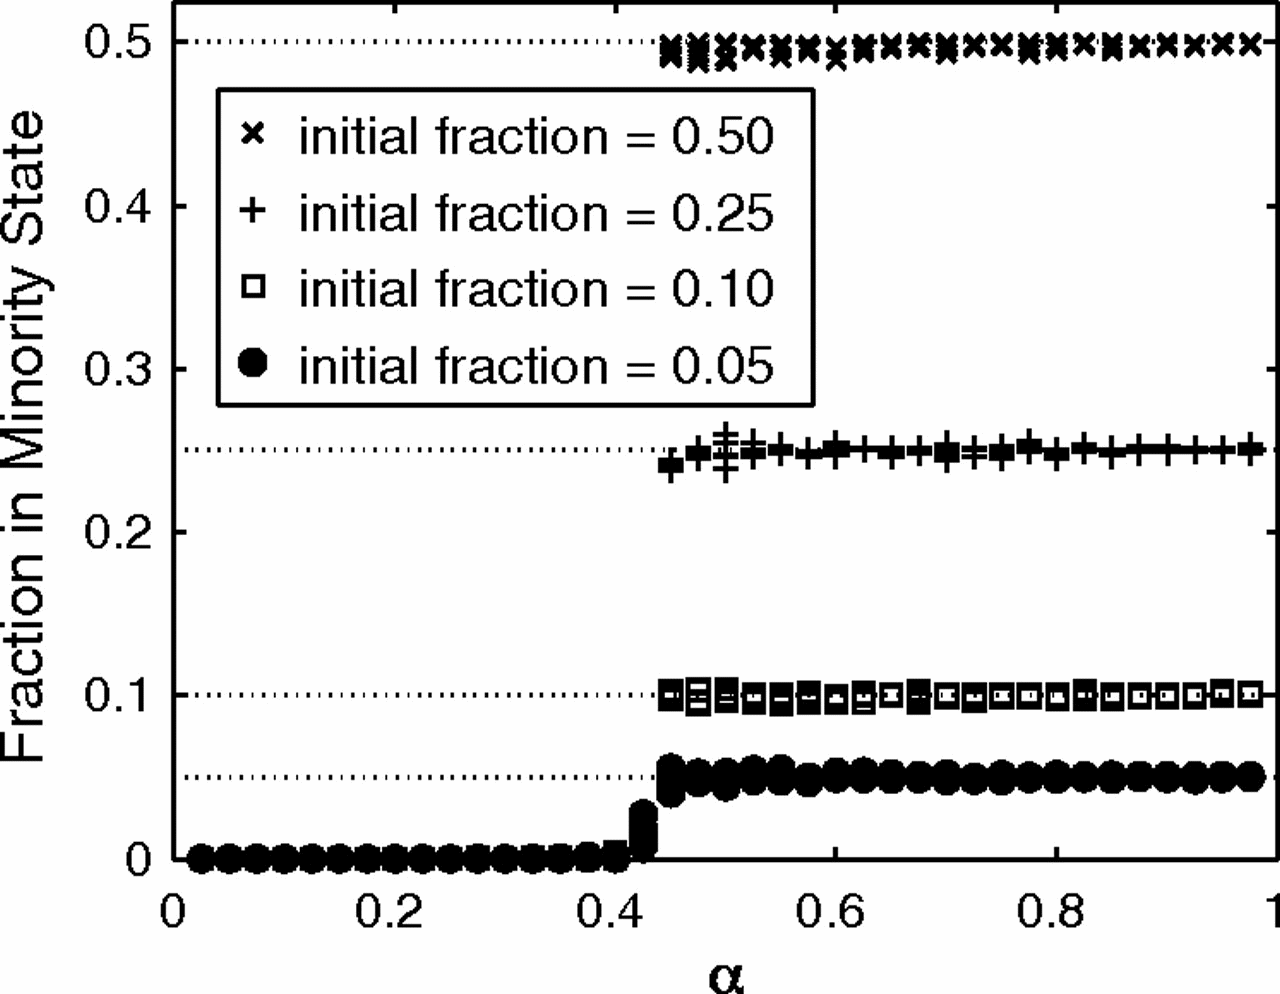
\includegraphics[height=65mm]{rwToSameBifDiag}
  \caption{Final minority fraction as a function of $\alpha$ and initial minority fraction (rewire-to-same), taken from \cite{durret:pnas12}.}
  \label{fig:durretRWtoSameBD}
\end{figure}

\begin{figure}
  \centering
  \subfloat[Only includes runs that have reached consensus]{
    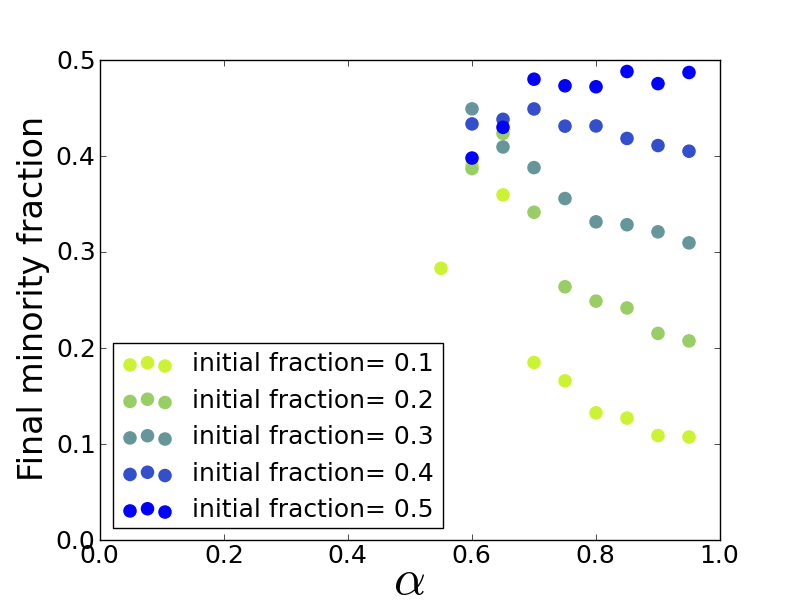
\includegraphics[width=72mm]{bifData_same_1000_4}
    \label{fig:rwSameA}
  }
  \hspace{3mm}
  \subfloat[Includes all runs, even if conflicts exist at the simulation's end] {
    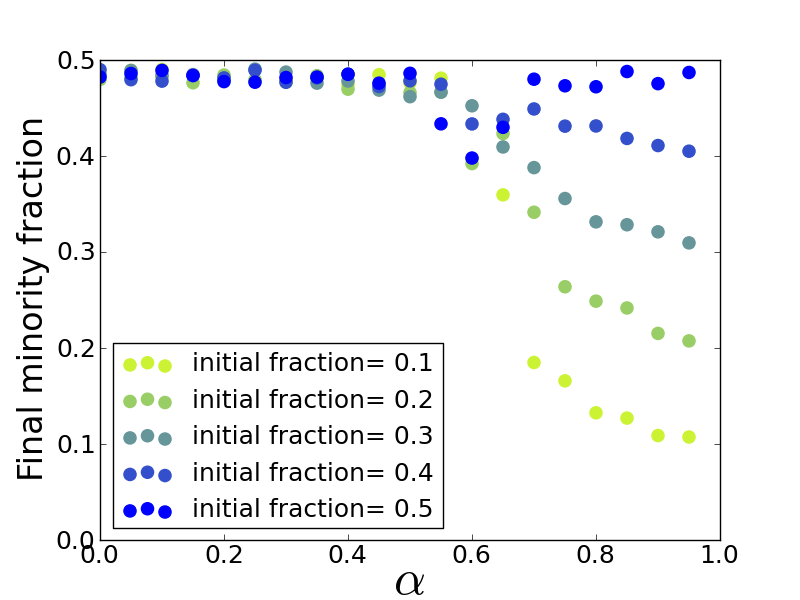
\includegraphics[width=72mm]{bifData_noConvergence_same_1000_4}
    \label{fig:rwSameB}
  }
  \caption{Final minority fraction as a function of $\alpha$ and initial minority fraction (rewire-to-same), results from our data.}
  \label{fig:myRWtoSameBD}
\end{figure}

\begin{figure}
  \centering
  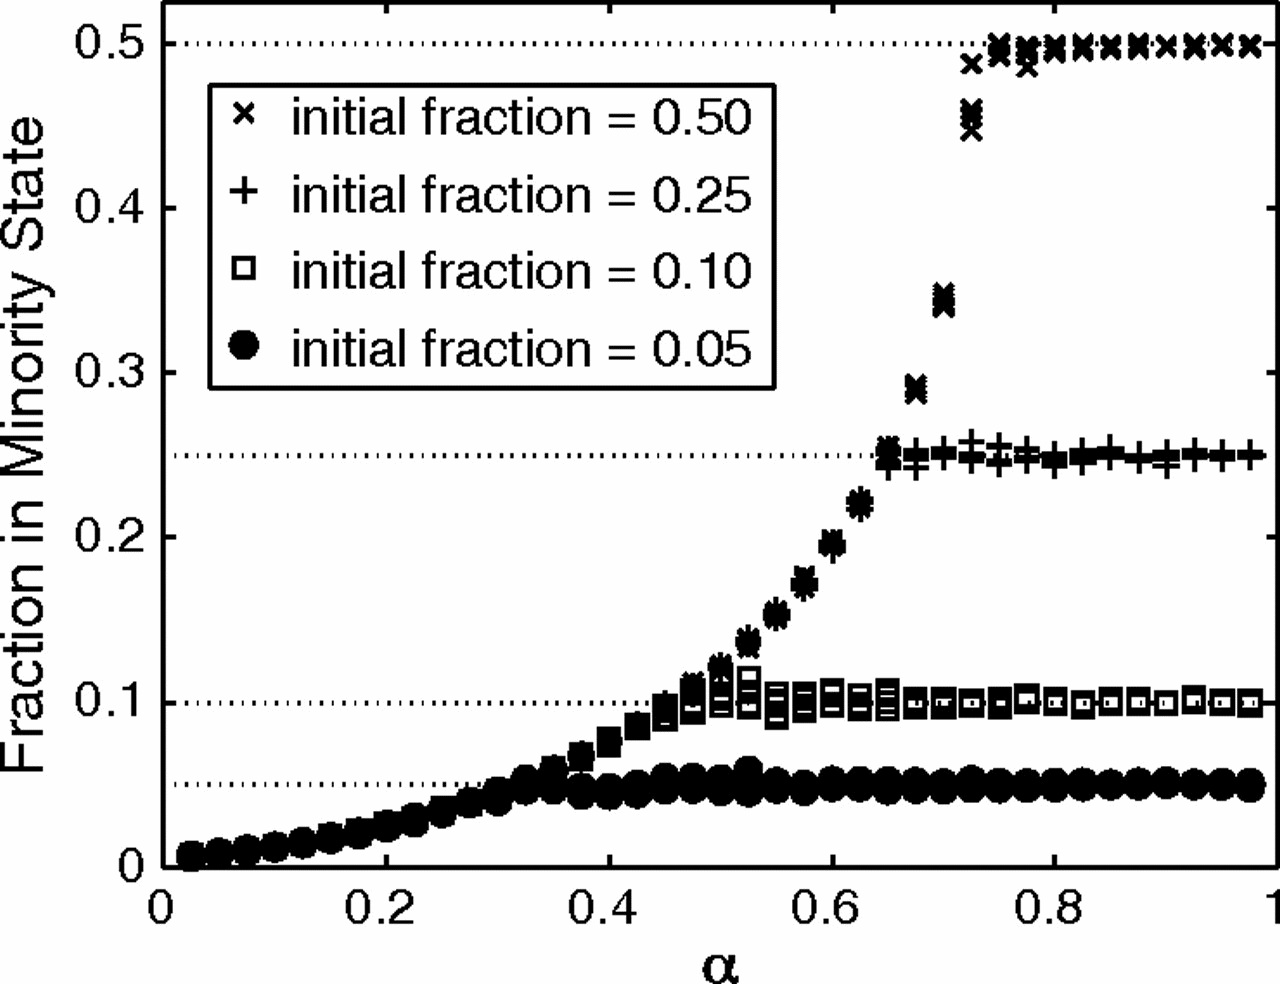
\includegraphics[height=65mm]{rwToRandomBifDiag}
  \caption{Final minority fraction as a function of $\alpha$ and initial minority fraction (rewire-to-random), taken from \cite{durret:pnas12}.}
  \label{fig:durretRWtoRandomBD}
\end{figure}

\begin{figure}
  \centering
  \subfloat[Runs that reached consensus]{
    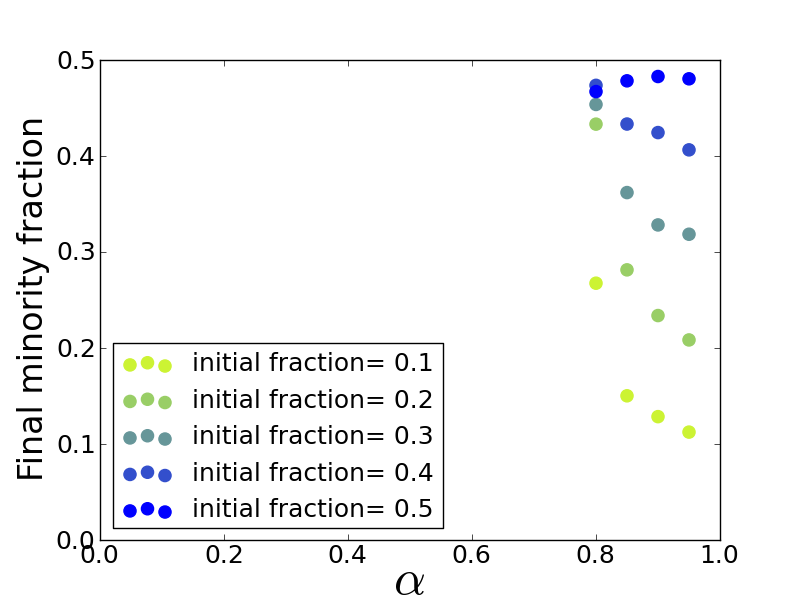
\includegraphics[width=72mm]{bifData_randomIneqJ_1000_4}
  }
  \hspace{3mm}
  \subfloat[All runs] {
    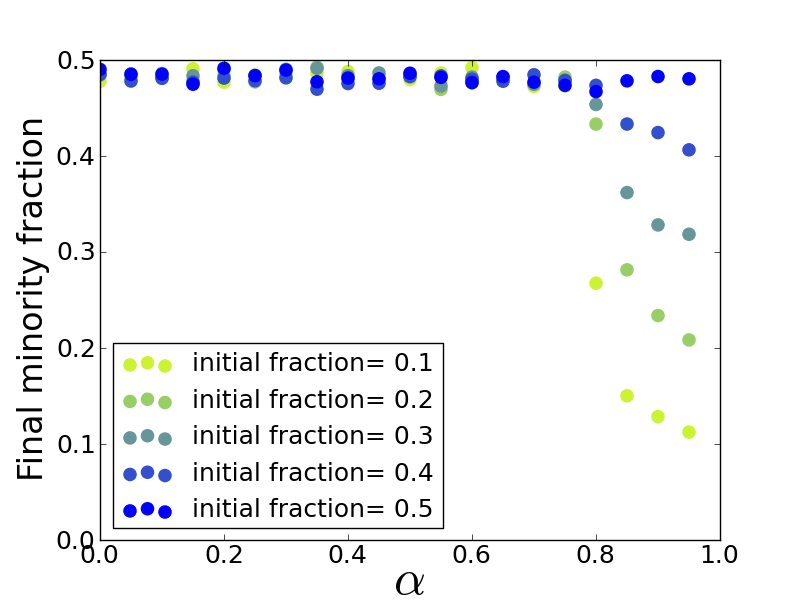
\includegraphics[width=72mm]{bifData_noConvergence_randomIneqJ_1000_4}
    \label{fig:myRWtoRandomFromDiffBDB}
  }
  \caption{Final minority fraction as a function of $\alpha$ and initial minority fraction (rewire-to-random), results from our data (from-different model).}
  \label{fig:myRWtoRandomFromDiffBD}
\end{figure}

\begin{figure}
  \centering
  \subfloat[Runs that reached consensus]{
    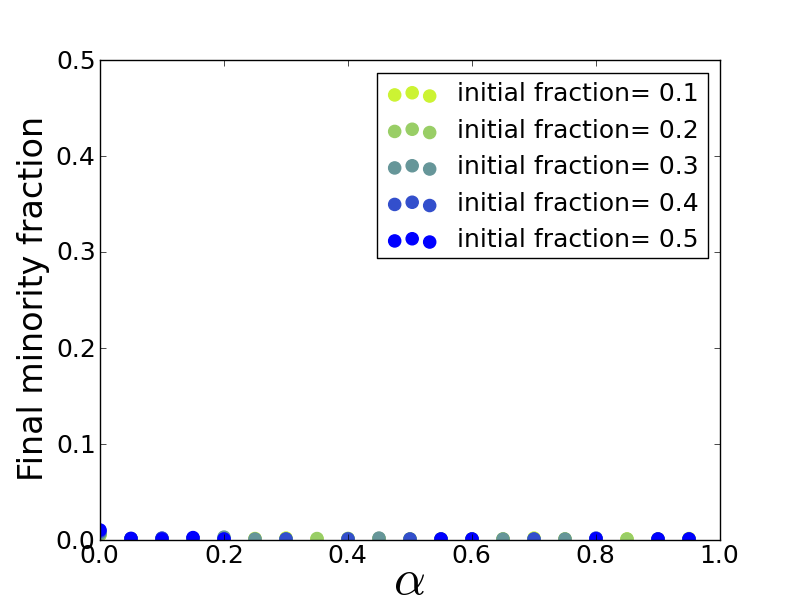
\includegraphics[width=72mm]{bifData_randomIeqJ_1000_4}
  }
  \hspace{3mm}
  \subfloat[All runs] {
    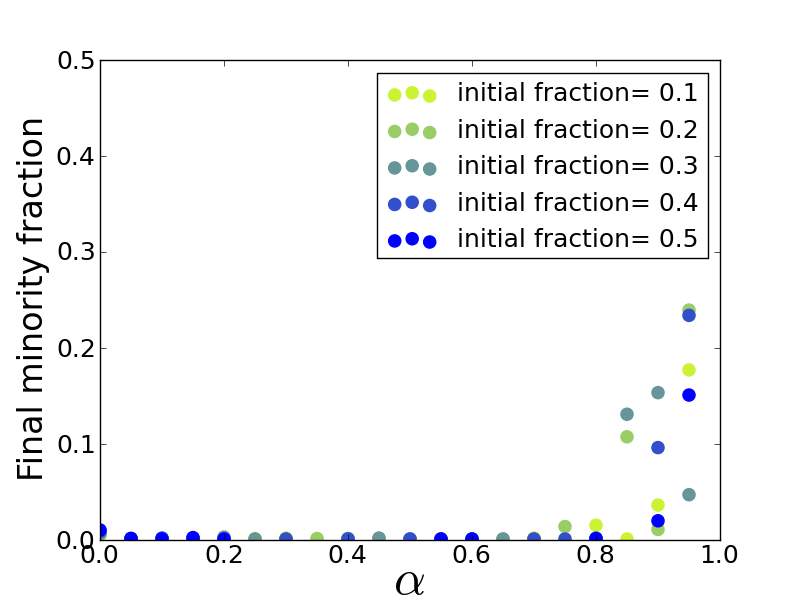
\includegraphics[width=72mm]{bifData_noConvergence_randomIeqJ_1000_4}
    \label{fig:myRWtoRandomFromAllBDB}
  }
  \caption{Final minority fraction as a function of $\alpha$ and initial minority fraction (rewire-to-random), results from our data (from-all model).}
  \label{fig:myRWtoRandomFromAllBD}
\end{figure}

\begin{figure}
  \centering
  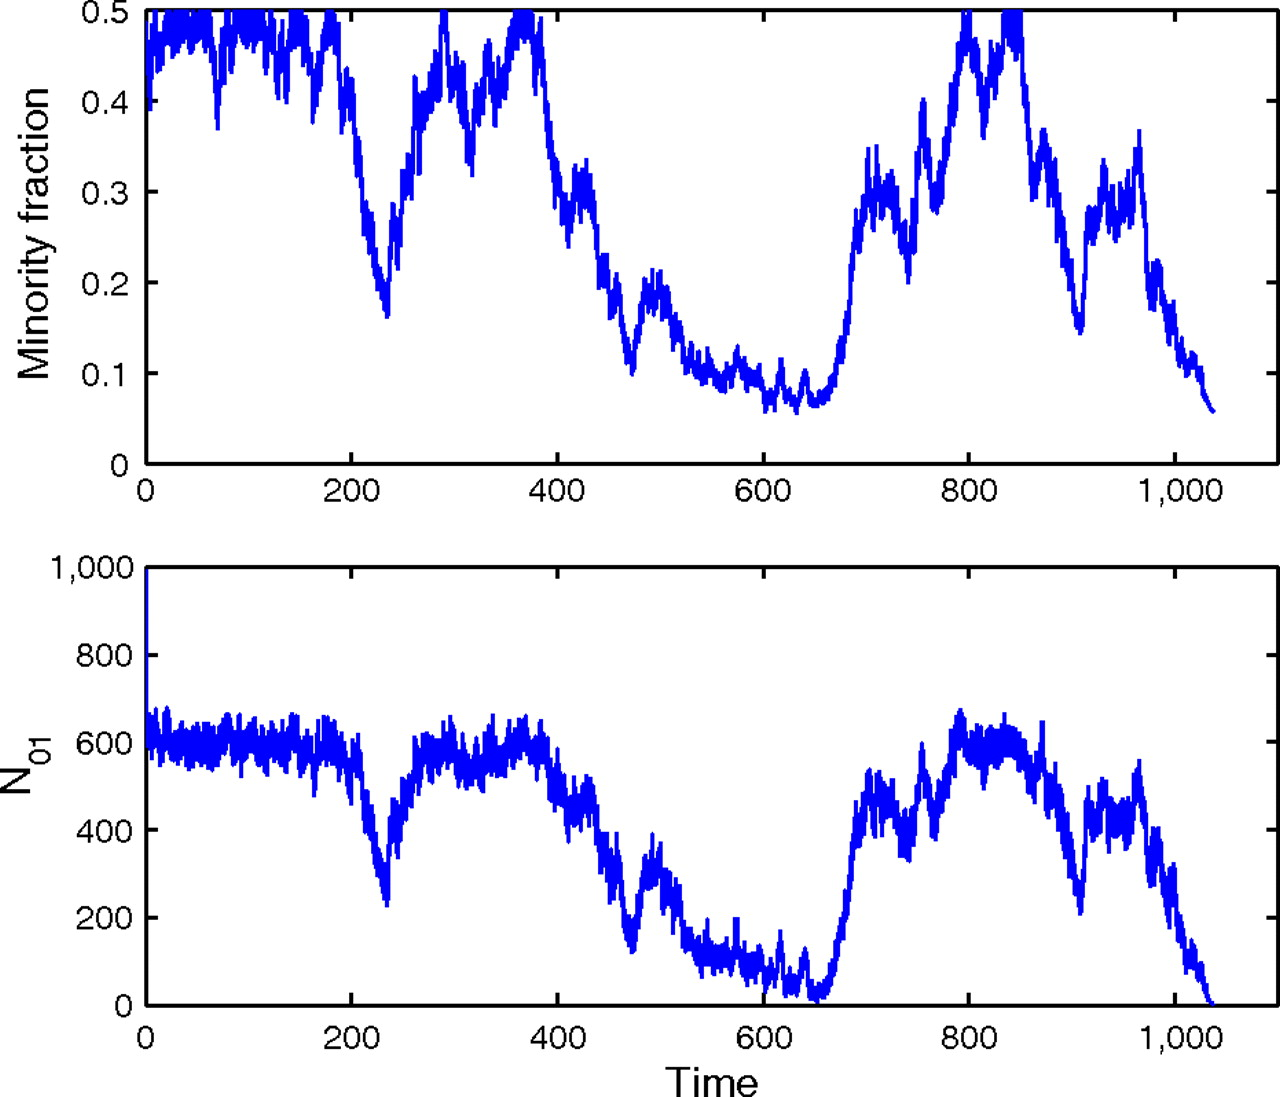
\includegraphics[height=65mm]{durretTimeCourses}
  \caption{Evolution of conflicting edges and minority fraction, taken from \cite{durret:pnas12}.}
  \label{fig:durretTimeCourses}
\end{figure}

\begin{figure}
  \centering
  \subfloat[Run that failed to reach consensus, $\alpha=0.5$.]{
    \includegraphics[width=72mm]{{graphStats_randomIneqJ_1000_4_0.5_0.5_0.5_noConsensus}.png}
    \label{fig:myIneqJTCsA}
  }
  \hspace{3mm}
  \subfloat[Run that reached consensus, $\alpha=0.8$.] {
    \includegraphics[width=72mm]{{graphStats_randomIneqJ_1000_4_0.8_0.5_0.5_consensus}.png}
  }
  \caption{Evolution of conflicting edges and minority fraction, results from our data (from-different model).}
  \label{fig:myIneqJTCs}
\end{figure}

\begin{figure}
  \centering
  \includegraphics[height=65mm]{{graphStats_randomIeqJ_1000_4_0.5_0.5_0.5_consensus}.png}
  \caption{Evolution of conflicting edges and minority fraction, results from our data (from-all model).}
  \label{fig:myIeqJTC}
\end{figure}

\begin{figure}
  \centering
  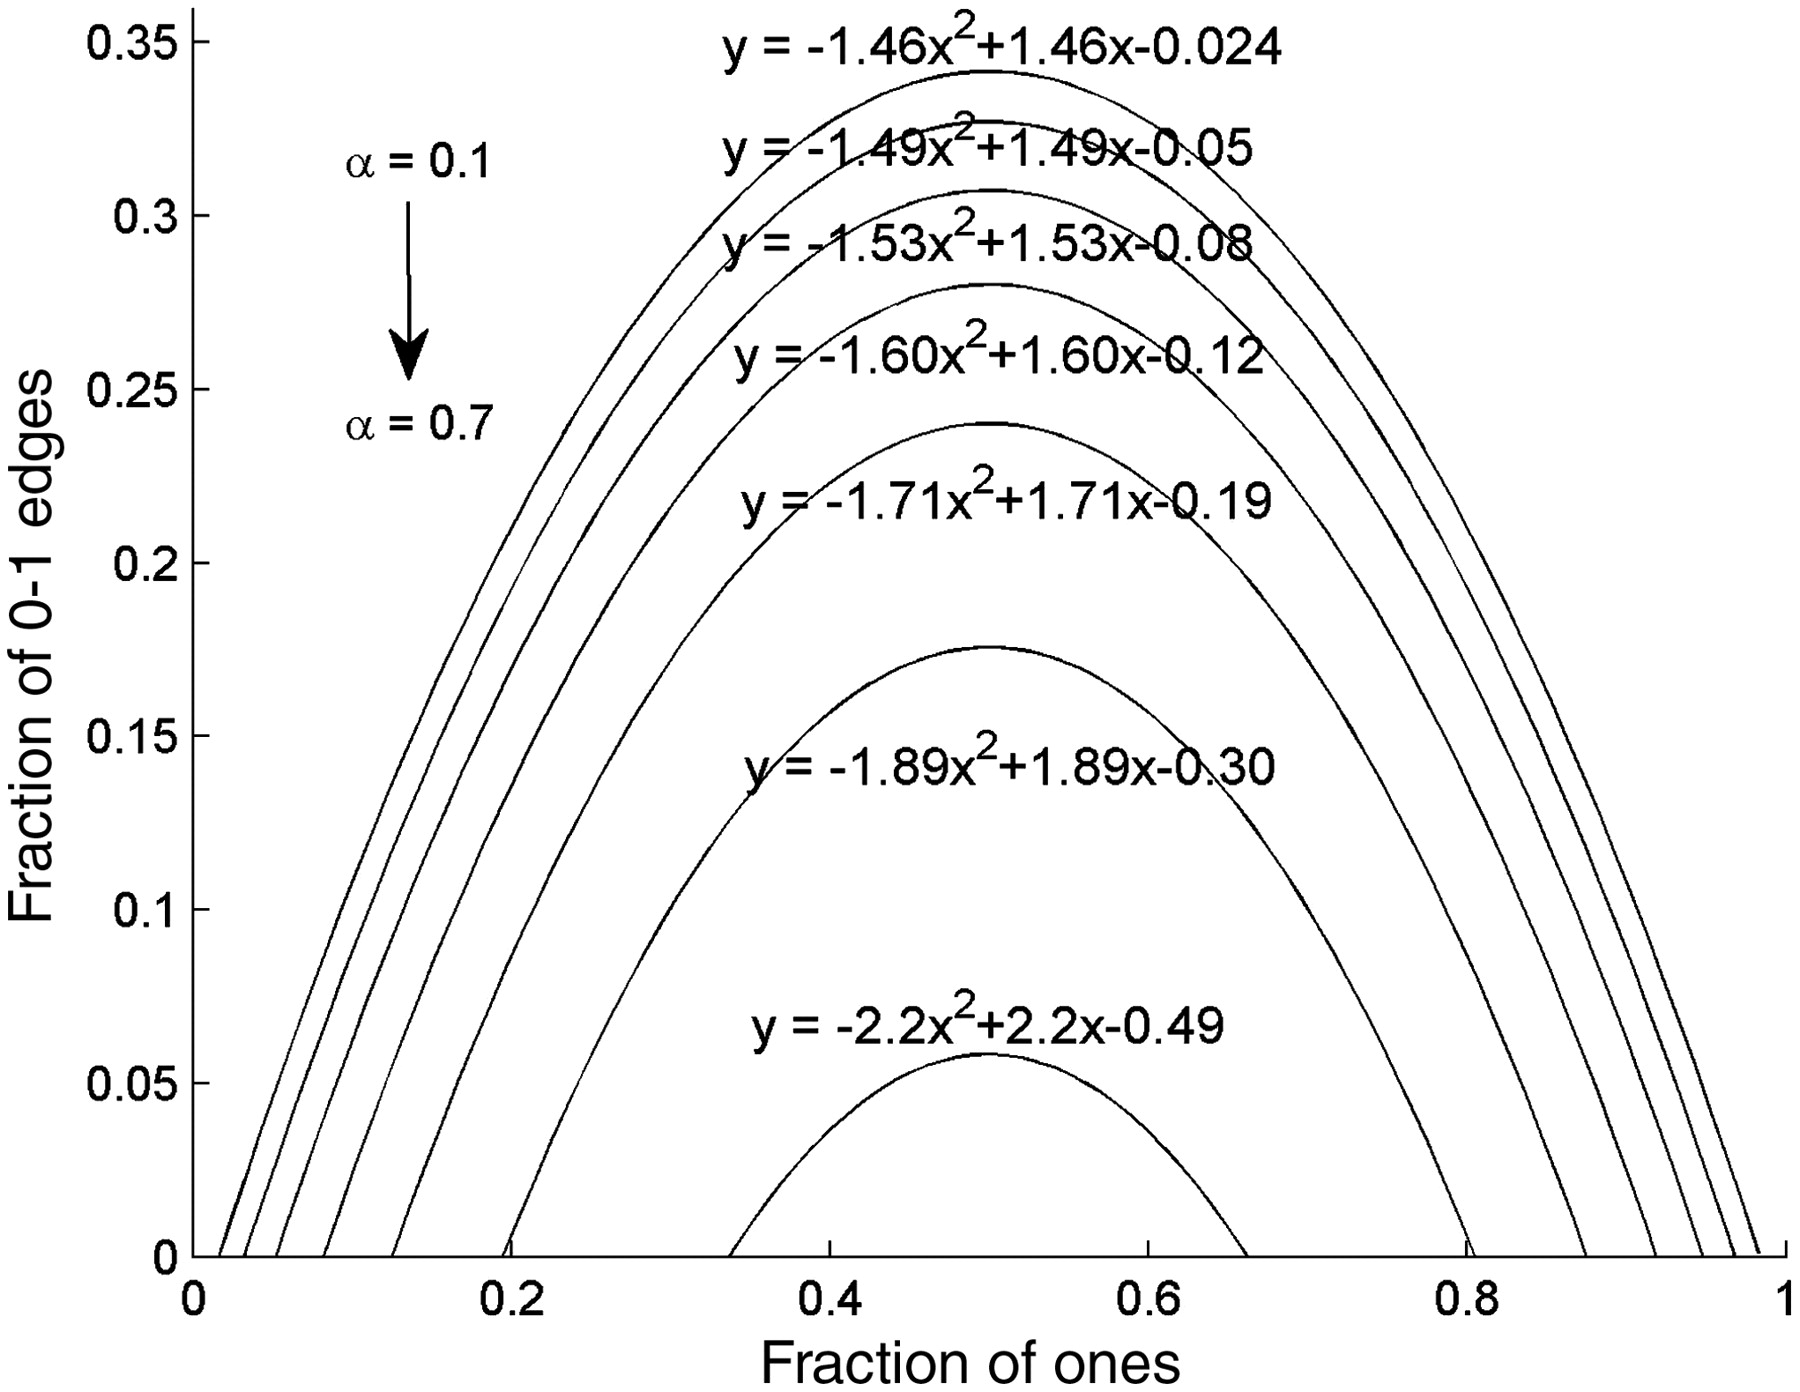
\includegraphics[height=65mm]{durretArcs}
  \caption{Random walk arcs as a function of $\alpha$, from \cite{durret:pnas12}.}
  \label{fig:durretArcs}
\end{figure}

\begin{figure}
  \centering
  \subfloat[From-different model]{
    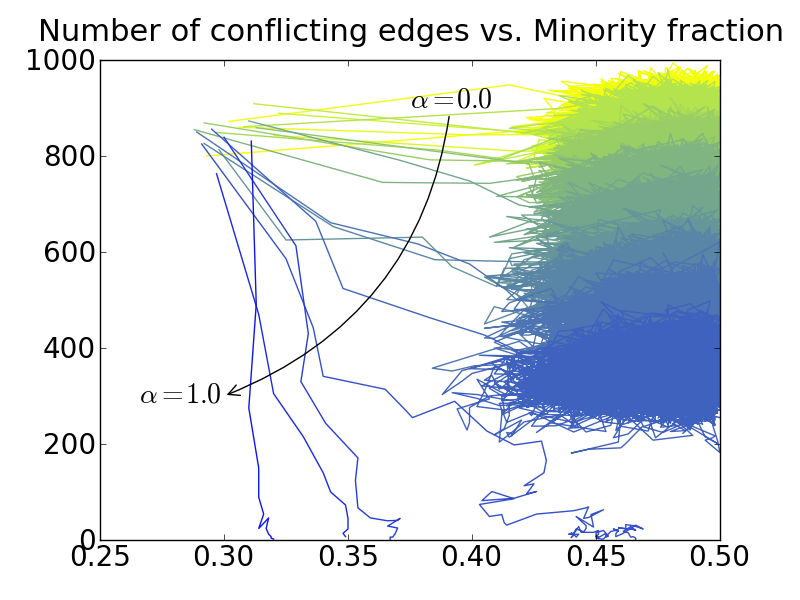
\includegraphics[width=72mm]{nData_randomIneqJ}
    \label{fig:myArcsA}
  }
  \hspace{3mm}
  \subfloat[From-all model] {
    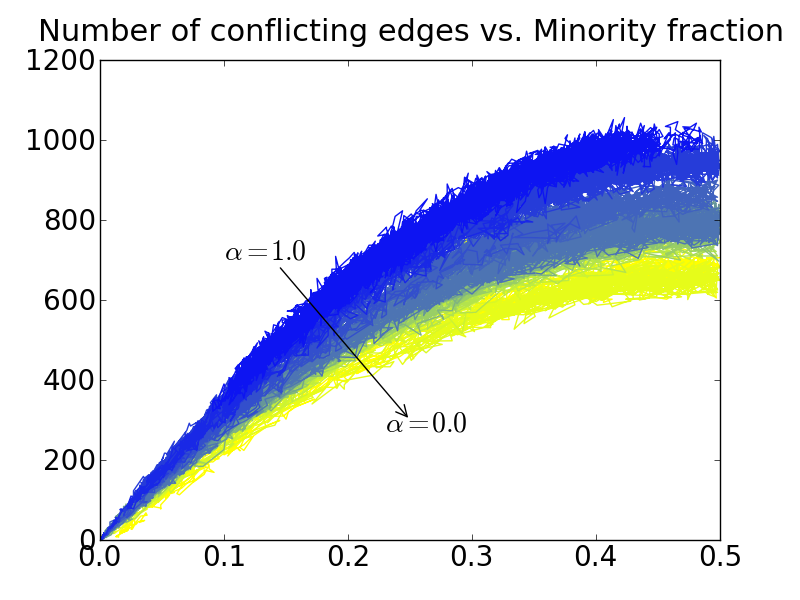
\includegraphics[width=72mm]{nData_randomIeqJ}
  }
  \caption{Random walk arcs from our two different implementations.}
  \label{fig:myArcs}
\end{figure}

\bibliographystyle{abbrv}
\bibliography{votingBib}
\end{document}


